\documentclass{article}
\input{boilerplate}

\begin{document}


\newcommand{\lectureTitle}{Generalizable RL for Neighborhood Battery Control in CityLearn}
\newcommand{\lectureDate}{Due: May 11th, 10:30 PM}

\textsc{COS435 / ECE433: Introduction to RL}
\vspace{1em} \hfill \lectureDate

\maketitle

\paragraph{Authors.} Grace Sun (\texttt{gs0625@princeton.edu}), Ammaar Alam (\texttt{ah0952@princeton.edu}), Erik Dyer (\texttt{ed1783@princeton.edu}) 

\paragraph{Link to GitHub Repo.} \url{https://github.com/Ammaar-Alam/cos435-citylearn}

\section{Introduction}

Buildings account for approximately 28\% of global CO$_2$ emissions \citep{iea2022buildings}, so coordinating distributed energy resources such as solar PV and battery storage is a control problem with real world stakes. As buildings electrify, they become both a source of grid stress and a potential source of flexibility. Batteries can absorb excess solar power, reduce peak demand, and shift consumption away from high carbon hours. This makes building energy management a natural testbed for reinforcement learning, where actions have delayed consequences and the controller must balance competing objectives over long horizons.

The CityLearn Challenge 2023 \citep{citylearn2023} formalizes this as a sequential decision making benchmark. At each hourly timestep, a controller observes a building level state (solar generation, net electricity demand, battery charge, temperature, and short horizon weather forecasts) and emits one continuous action $a_t \in [-1, +1]$ representing a charge or discharge per building. The environment scores the resulting neighborhood trajectory using five weighted key performance indicators (KPIs). They are
\begin{enumerate}
    \item Electricity cost, the normalized cost of electricity consumed by buildings in the neighborhood. The goal of the agent is to shift loads to cheaper periods, charging batteries when prices are low and discharging when prices are high.
    \item Carbon emissions, a building level KPI measuring emissions based on each building's electricity consumption. Agents reduce emissions by shifting demand to hours when the grid is running on cleaner or less carbon intense energy. 
    \item Daily peak demand. A neighborhood level KPI that measures the maximum electricity demand reached within each day, averaged across all days. High peak demand in urban areas increases electricity price and can cause grid instability or even blackouts.
    \item Thermal discomfort, a building level KPI that quantifies how far indoor temperatures deviate from occupants' specified comfort band of preferred temperature.
    \item Thermal resilience loss, a KPI introduced in Phase II of CityLearn 2023 to measure how well buildings maintain thermal comfort during power outages.
\end{enumerate}
To get a high score, a controller has to respond to solar and demand signals, and make complex decisions like how much capacity to reserve for future peaks, whether to prioritize carbon or cost at a given hour, and how to avoid actions that improve one KPI at the expense of another.

The main challenge is generalization. A learned policy can overfit on the training split and degrade on held out conditions. It can also overfit architecturally. 
A policy whose input and output layers are fixed to three buildings cannot run on a six building neighborhood. Rule based control (RBC) sidesteps both failure modes by encoding human priors rather than fitting data, which helps explain why the strongest prior entries, such as the 2023 competition winner CHESCA \citep{pinto2024citylearn}, have favored hierarchical optimization over learned policies. Prior RL approaches to CityLearn have struggled with three recurring gaps. Reward signals do not directly match the composite evaluation criterion, single run results overstate reliability, and fixed topology architectures cannot adapt to neighborhoods of different sizes. Our work directly addresses all three.

We ask whether a systematic RL pipeline can outperform RBC on held out evaluation data while remaining portable to building configurations never seen during training. Rather than searching for a single best hyperparameter setting, we run a controlled ablation across two algorithms (PPO and SAC), two control topologies (centralized and shared parameter decentralized), and three reward variants, using multiseed runs ($n = 3$--$10$) and reporting confidence intervals throughout. Section~\ref{sec:related} reviews related work on CityLearn and continuous control algorithms; Section~\ref{sec:methods} describes our experimental design; Section~\ref{sec:results} presents results; and Section~\ref{sec:discussion} discusses findings and limitations. Our main contributions are

\begin{itemize}
    \item SAC with a reward aligned to the official scoring terms reduces the RBC composite score by 48\% on the local evaluation dataset and by 40\% on the released held out phase 2 splits.
    \item Shared parameter decentralized training/execution (shared-DTDE) is the only topology portable to the 6 building phase 3 held out splits; among portable policies, SAC-DTDE outperforms PPO-DTDE on phase 3 (0.774 vs.\ 0.843).
    \item A reward design ablation shows that matching the official scoring terms improves local performance, while adding battery smoothness penalties improves held out phase 2 generalization.
\end{itemize}

\section{Related Work}\label{sec:related}

The CityLearn environment \citep{vazquez2020citylearn, citylearnrepo} has been the platform for multiple competition tracks on building level energy management. The strongest entries in the 2023 challenge combined explicit forecasting, hierarchical control, and optimization rather than end to end learned policies. CHESCA \citep{pinto2024citylearn} achieved the top score by first optimizing individual building behavior and then refining decisions through a community level controller, giving it both scalability and explicit structure. The 2023 second place solution \citep{zheng2025optimizing} combined learned forecasts (linear regression, k-NN, and LightGBM) with building level and microgrid level model predictive control. Earlier work similarly found that optimization with online adaptation is highly competitive while remaining interpretable \citep{khattar2023winning}. Collectively, these results motivate a narrower question of which design choices make a simple RL baseline credible, reproducible, and portable, and how much of the gap to optimization they can close.

The two algorithms we evaluate are PPO \citep{schulman2017proximal} and SAC \citep{haarnoja2018soft}. PPO is a widely used on policy method with a clipped surrogate objective that stabilizes training across a range of continuous control tasks. SAC is an off policy actor critic that adds entropy regularization, improving sample efficiency and reducing sensitivity to reward scaling. Properties that are especially valuable in the sample limited continuous control setting of battery dispatch. We use Stable-Baselines3 \citep{raffin2021stable} for centralized variants and a custom shared parameter stack for decentralized execution. Building energy management poses specific challenges for both algorithms. Episodes span a full year of hourly operations over 8,760 steps, rewards from the multi KPI scoring formula have different timescales like in the case where thermal comfort is instantaneous while peak demand accumulates over days, and actions in a shared battery schedule create delayed effects that are hard to attribute to individual timesteps. These properties favor off policy methods with long replay memory, and motivate our reward design ablation as a controlled experiment in aligning the training signal with the evaluation criterion.

Centralized versus decentralized control for building energy management has been studied directly in prior work. \citet{kathirgamanathan2021centralised} compared centralized and decentralized RL for battery control in a smart grid setting and found tradeoffs between coordination quality and scalability. Centralized policies have access to all agents' observations and can optimize a joint action, but they do not generalize to different numbers of agents at test time. Parameter sharing in decentralized policies offers a practical middle ground. Buildings are treated as instances of the same control problem, a single network is trained on experience pooled across all buildings, and the resulting checkpoint can run on any neighborhood size. Our work extends this comparison by evaluating the topology tradeoff across both same size and cross size held out splits under a systematic reward design ablation, making the generalization cost of each choice quantitatively visible.

\section{Methods}\label{sec:methods}

We compare two RL algorithms across two control topologies and three reward formulations, evaluated on local and released held out splits from the CityLearn 2023 competition.

\paragraph{Environment.} We use the CityLearn Gymnasium environment \citep{vazquez2020citylearn, citylearnrepo} in its 2023 competition configuration of a 3 building neighborhood with rooftop solar PV and battery storage at each building. Observations include time of day encodings, normalized net electricity demand, solar generation, battery state of charge, and short horizon forecasts. The composite score (lower is better) is a normalized weighted average of five KPI ratios, each comparing agent performance to a do nothing baseline.

\paragraph{Control topologies.} We evaluate two architectures. In the centralized topology, one neural network receives the concatenated observations of all three buildings and emits a three dimensional joint action. This gives the policy full neighborhood information but fixes the network dimensions to the training building count. In the shared-DTDE topology, one policy network is applied independently to each building's local observation window. Buildings act without observing one another at inference time, while training reuses experience across buildings through shared parameters and, for SAC, a shared replay buffer. Because the policy is applied per building, the same checkpoint runs on any number of buildings by making $N$ independent forward passes.

\paragraph{Algorithms and architecture.}
\begin{itemize}
    \item PPO \citep{schulman2017proximal}  On policy proximal policy optimization with a clipped surrogate objective. We implement centralized PPO with Stable-Baselines3 \citep{raffin2021stable} and a custom shared-DTDE variant with per building embeddings. The shared-DTDE PPO policy uses a 2 layer MLP (256 hidden units per layer) applied per building; the rollout buffer pools experience across all buildings. We sweep learning rates over $\{10^{-4}, 3\times10^{-4}\}$ across 10 seeds and select the best per seed on the local validation split.
    \item SAC \citep{haarnoja2018soft}  Off policy soft actor critic with entropy regularization. SAC reuses transitions through replay, which is useful in sample limited continuous control settings. Both the centralized and shared-DTDE SAC variants use 2 layer MLP actor and critic networks (256 hidden units), a replay buffer of size $10^6$, and automatic entropy tuning. We implement centralized SAC (5 seeds) and a shared-DTDE SAC pilot (3 seeds), the latter using a shared replay buffer that pools transitions from all buildings.
\end{itemize}

All policies train for 500K, or 1M environment steps. Centralized policies treat the 3 building tuple as a single environment step; shared-DTDE variants accumulate one transition per building per environment step, effectively multiplying the transition count by the number of buildings. Checkpoints are saved every 50K steps and the final checkpoint (not the best validation checkpoint) is used for evaluation, which avoids implicit validation leakage.

\paragraph{Reward design.}
The default CityLearn reward is a negative net consumption proxy, but the competition ranks submissions using a multiterm composite score. We test three reward variants

\begin{itemize}
    \item \texttt{reward\_v0} (baseline): The environment's built-in default reward. This is a sanity check because the training signal does not directly match the evaluation criterion.
    \item \texttt{reward\_v1}  A handcrafted 8 term weighted penalty mirroring the official 2023 scoring formula. Component weights are thermal discomfort ($0.30$), outage discomfort ($0.15$), unserved energy ($0.15$), carbon emissions ($0.10$), and four peak/ramping terms at $0.075$ each. This trains the agent directly on the terms used for evaluation.
    \item \texttt{reward\_v2}: Extends \texttt{reward\_v1} with two battery smoothness penalties, which are a penalty proportional to absolute SoC change per step ($0.05 \cdot |\Delta \text{SoC}|$) and a binary penalty for charge to discharge sign flips ($0.05 \cdot \mathbf{1}[\text{sign flip}]$). These terms discourage control that exploits the training split but generalizes poorly.
\end{itemize}

The reward variant ablation is fully crossed for centralized SAC. PPO uses \texttt{reward\_v2} throughout because of compute constraints.

\paragraph{Evaluation protocol.} We evaluate in three regimes. Local \texttt{public\_dev} is our primary tuning environment (one 3-building dataset available during development). Released phase 2 online-eval contains three held out 3 building datasets, testing same topology generalization. Released phase 3 contains three held out 6 building datasets, testing cross size generalization. Only shared-DTDE policies can run on phase 3. We report seed averaged means with 95\% confidence intervals throughout.

\paragraph{Implementation and reproducibility.} All reported numbers come from saved checkpoints evaluated against named split configs, not the last training step scores. We maintain seed inventories and aggregation scripts that write directly to \texttt{submission/results/} and \texttt{submission/figures/}. This separation makes coverage gaps explicit. For example, the 3 seed SAC-DTDE pilot is flagged as such for every result table.

\section{Results}\label{sec:results}

We organize results around the three evaluations of local tuning performance, same topology held out generalization during phase 2, and cross size generalization during phase 3. All figures and tables report seed averaged means with 95\% confidence intervals and error bars.

\begin{figure}[t]
    \centering
    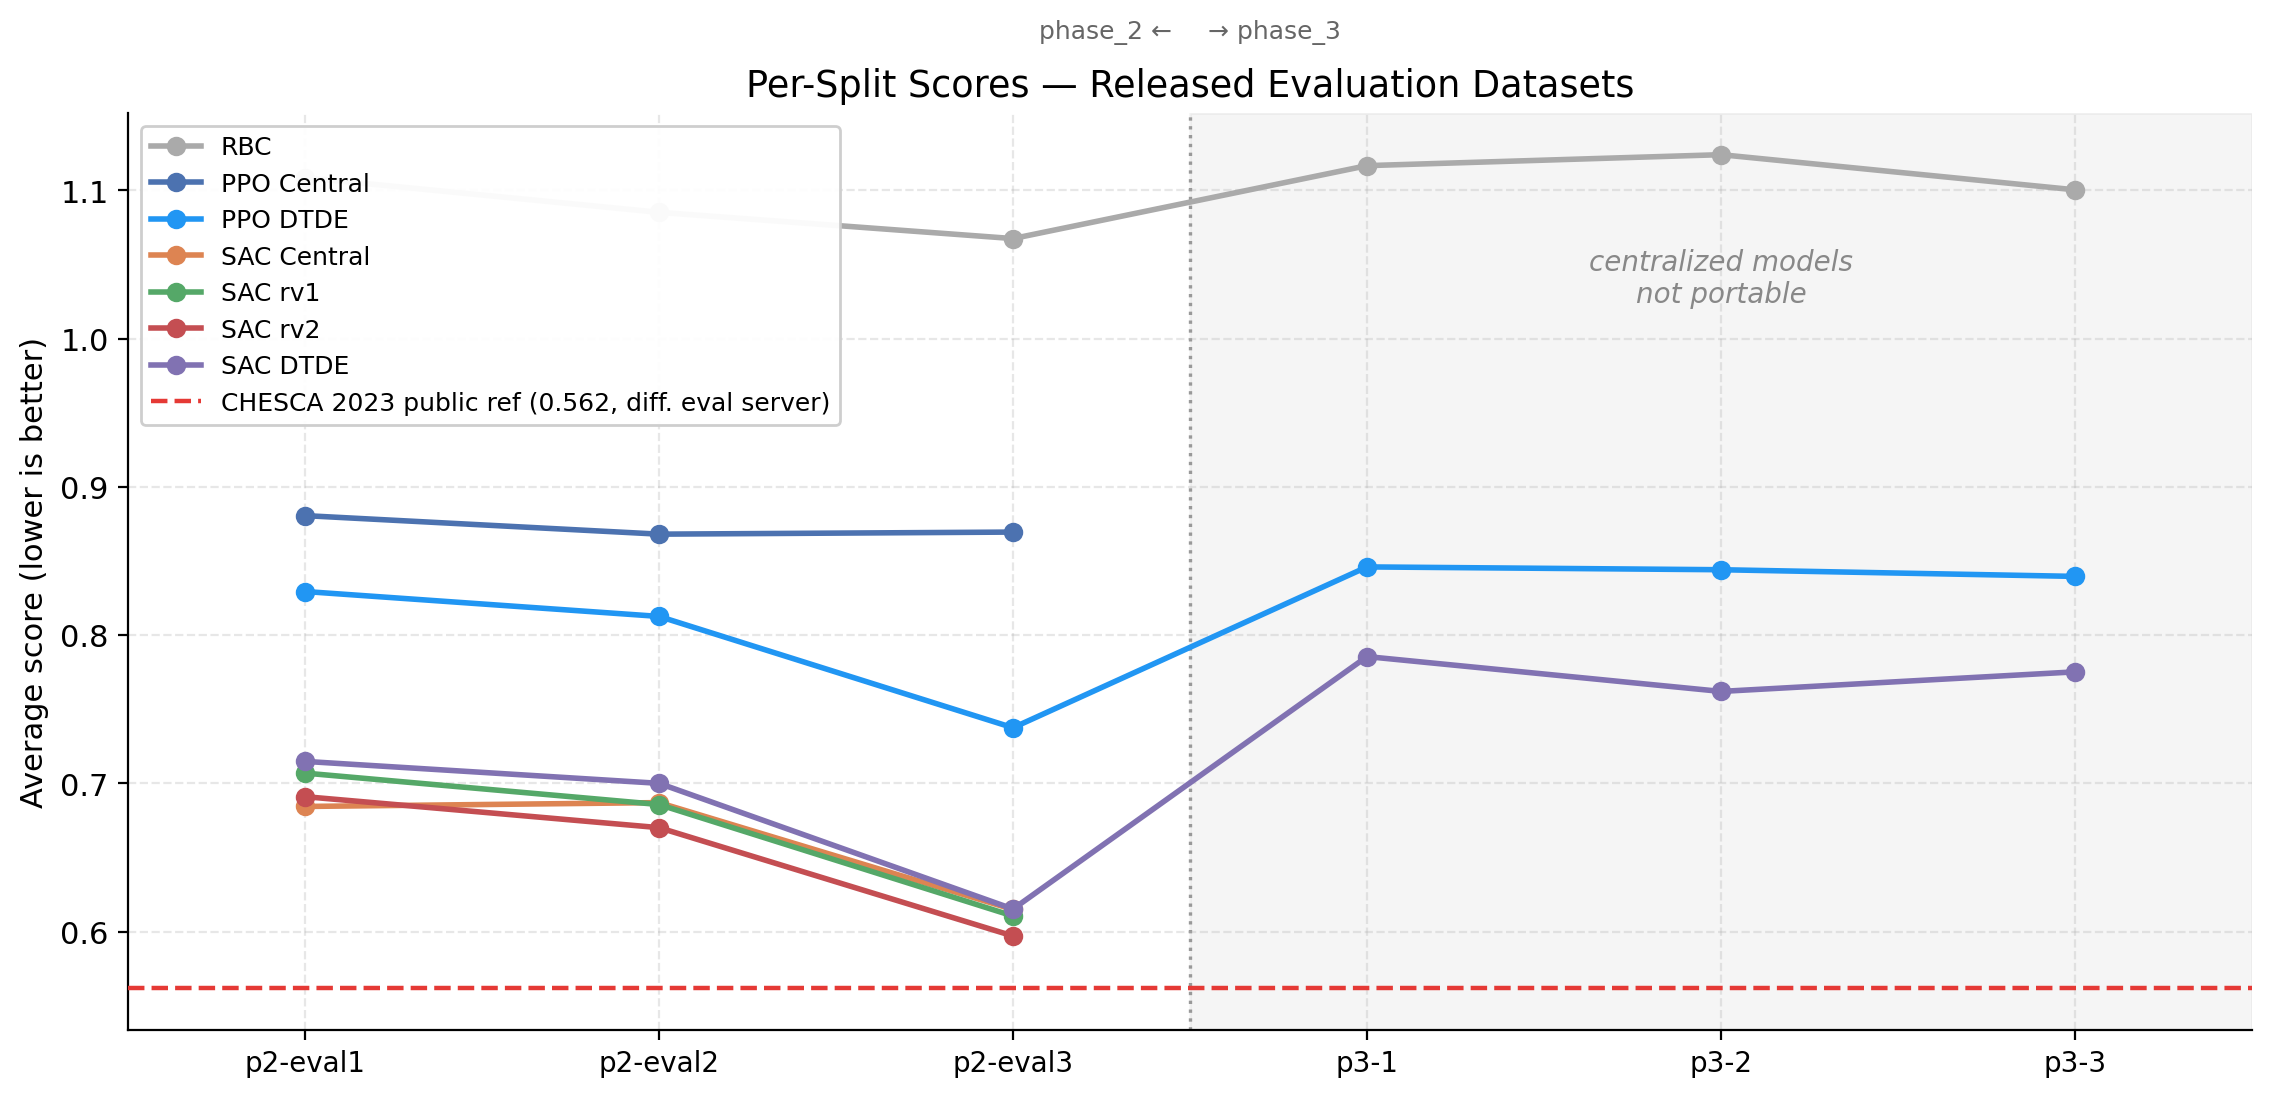
\includegraphics[width=\linewidth]{figures/per_split_scores.png}
    \caption{
        \texttt{average\_score} (lower is better) on six released held out evaluation datasets. Left panel  three \texttt{phase\_2\_online\_eval} splits (3 building). Right panel (shaded)  three \texttt{phase\_3} splits (6 building). Centralized policies cannot execute on phase 3 splits due to input/output size mismatch. SAC-DTDE achieves the best phase 3 mean (0.774), confirming that shared parameter decentralization is the only topology that enables cross size generalization. The dashed line at 0.562 is the CHESCA 2023 public leaderboard reference. Note that it is from a private evaluator and shown for benchmark context, not for direct comparison.
    }
    \label{fig per_split}
\end{figure}

\paragraph{Local evaluation.} Table~\ref{tab local} summarizes results on the local \texttt{public\_dev} split. The local RBC baseline scores 1.023, and every RL method improves on it. The best local variant is SAC centralized \texttt{reward\_v1} at $0.527 \pm 0.011$ (5 seeds), a 48.4 reduction relative to RBC. SAC \texttt{reward\_v2} ($0.536 \pm 0.016$) and the SAC baseline ($0.554 \pm 0.009$) trail by 1--3 points, indicating that reward alignment helps but is not the sole driver. SAC shared-DTDE scores $0.569 \pm 0.018$ (3 seed pilot), modestly behind centralized SAC. The decentralized controller sees only per building observations and cannot jointly coordinate charge/discharge across the neighborhood. PPO variants are substantially weaker (0.777--0.883), consistent with SAC's expected advantage in continuous control tasks from off policy replay and entropy regularization.

\begin{table}[h]
\centering
\small
\begin{tabular}{lcccc}
\toprule
\textbf{Method} & \textbf{Seeds} & \textbf{Mean $\pm$ Std} & \textbf{95\% CI} & \textbf{\% vs.\ RBC} \\
\midrule
Local RBC baseline        & 1  & 1.023 $\pm$ 0.000 & ---   & --- \\
PPO centralized baseline  & 6  & 0.883 $\pm$ 0.011 & 0.012 & $-$13.7\% \\
PPO shared-DTDE \texttt{rv2}    & 10 & 0.777 $\pm$ 0.037 & 0.026 & $-$24.0\% \\
SAC centralized baseline  & 5  & 0.554 $\pm$ 0.009 & 0.011 & $-$45.8\% \\
SAC centralized \texttt{rv2}    & 5  & 0.536 $\pm$ 0.016 & 0.020 & $-$47.6\% \\
SAC centralized \texttt{rv1}    & 5  & 0.527 $\pm$ 0.011 & 0.014 & $-48.4\%$ \\
SAC shared-DTDE \texttt{rv2}    & 3  & 0.569 $\pm$ 0.018 & 0.044 & $-$44.4\% \\
\bottomrule
\end{tabular}
\caption{Local \texttt{public\_dev} results (lower is better). \% vs.\ RBC = percentage improvement over the local RBC baseline score of 1.023.}
\label{tab local}
\end{table}

\paragraph{Held out phase 2 generalization.} The released phase 2 splits change the weather and demand traces while keeping the 3 building topology. Absolute scores shift, but the local rank ordering mostly persists. RBC rises to 1.087 (mean over 3 splits). SAC centralized \texttt{reward\_v2} achieves the best RL result at $0.653 \pm 0.043$ (15 eval jobs, 5 seeds), a 40\% improvement over held out RBC. Importantly, \texttt{rv2} outperforms \texttt{rv1} here despite losing locally (0.653 vs.\ 0.668). The smoothness penalties reduce overfitting to the development split, a consistent pattern suggesting that the SoC change and sign flip penalties act as a form of behavioral regularization that transfers better across weather and demand conditions. SAC shared-DTDE scores $0.677 \pm 0.047$, within 2 points of centralized SAC despite operating on only per-building observations. PPO variants retain their advantage over RBC (0.793 and 0.873) while remaining well below SAC. The generalization gap (local score vs.\ phase-2 mean) for SAC centralized is approximately 0.12--0.14 points, compared to 0.02--0.05 for PPO shared-DTDE---smaller in absolute terms for PPO but from a much weaker starting point, so SAC remains the stronger held out controller.

\begin{figure}[h]
    \centering
    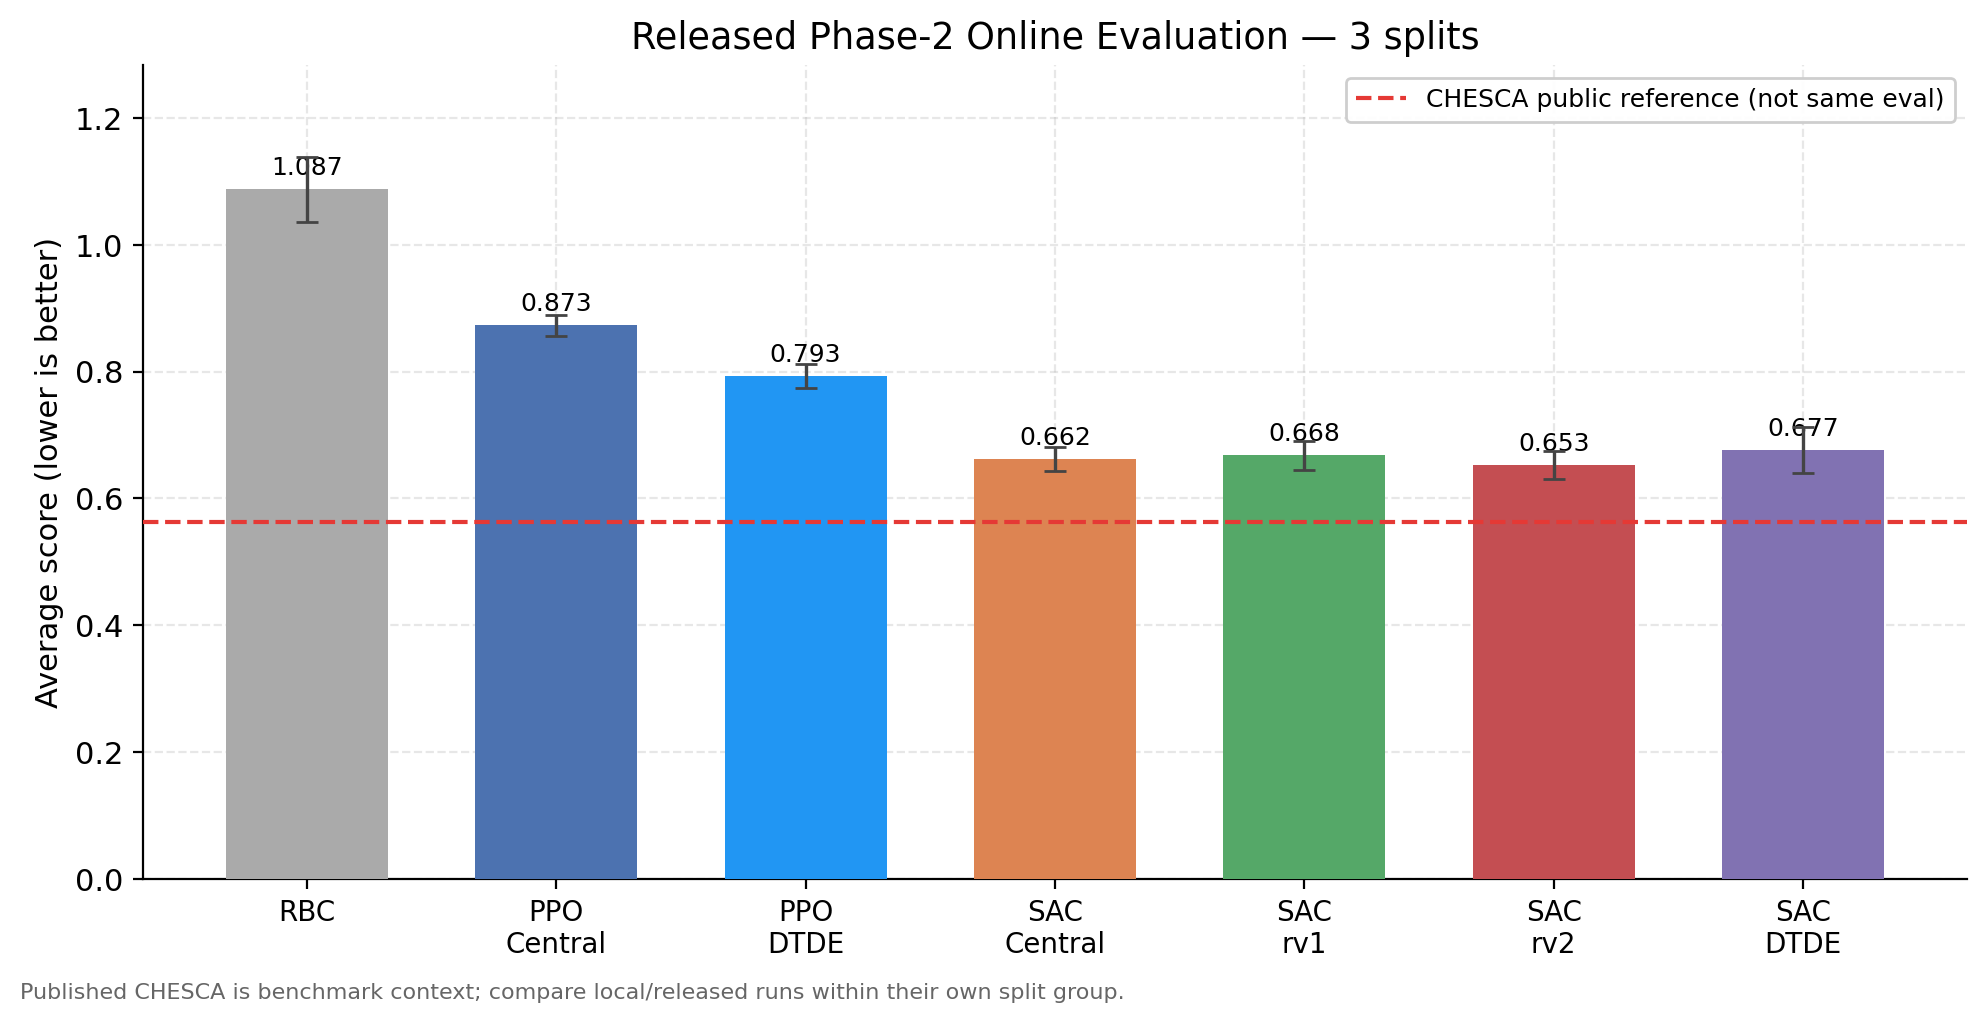
\includegraphics[width=\linewidth]{figures/cross_split_comparison.png}
    \caption{
        Method comparison across the local \texttt{public\_dev} split and the three released \texttt{phase\_2\_online\_eval} splits. Error bars show 95\% confidence intervals. All RL methods beat RBC on every split; SAC variants lead consistently, and the smoothness-regularized \texttt{reward\_v2} variant achieves the best held-out phase-2 performance despite a small local regression.
    }
    \label{fig cross_split}
\end{figure}

\paragraph{Cross size generalization to phase 3.} The released phase 3 splits expand the cluster from 3 to 6 buildings, providing the strictest generalization test. Centralized policies fail outright here  feeding a 6 building observation to a 3 building checkpoint is a shape mismatch, not a performance question. Among portable methods, SAC shared-DTDE achieves 0.774 (mean over 3 splits, 9 eval jobs), compared to 0.843 for PPO shared-DTDE and 1.114 for RBC. Shared-DTDE treats buildings as repeated instances of the same local control problem, so the same forward pass applies independently to each building's observation and no architectural change is needed. SAC-DTDE's advantage over PPO-DTDE widens slightly on phase 3, likely because additional buildings supply more diverse per building replay data for the off policy learner.

\begin{figure}[h]
    \centering
    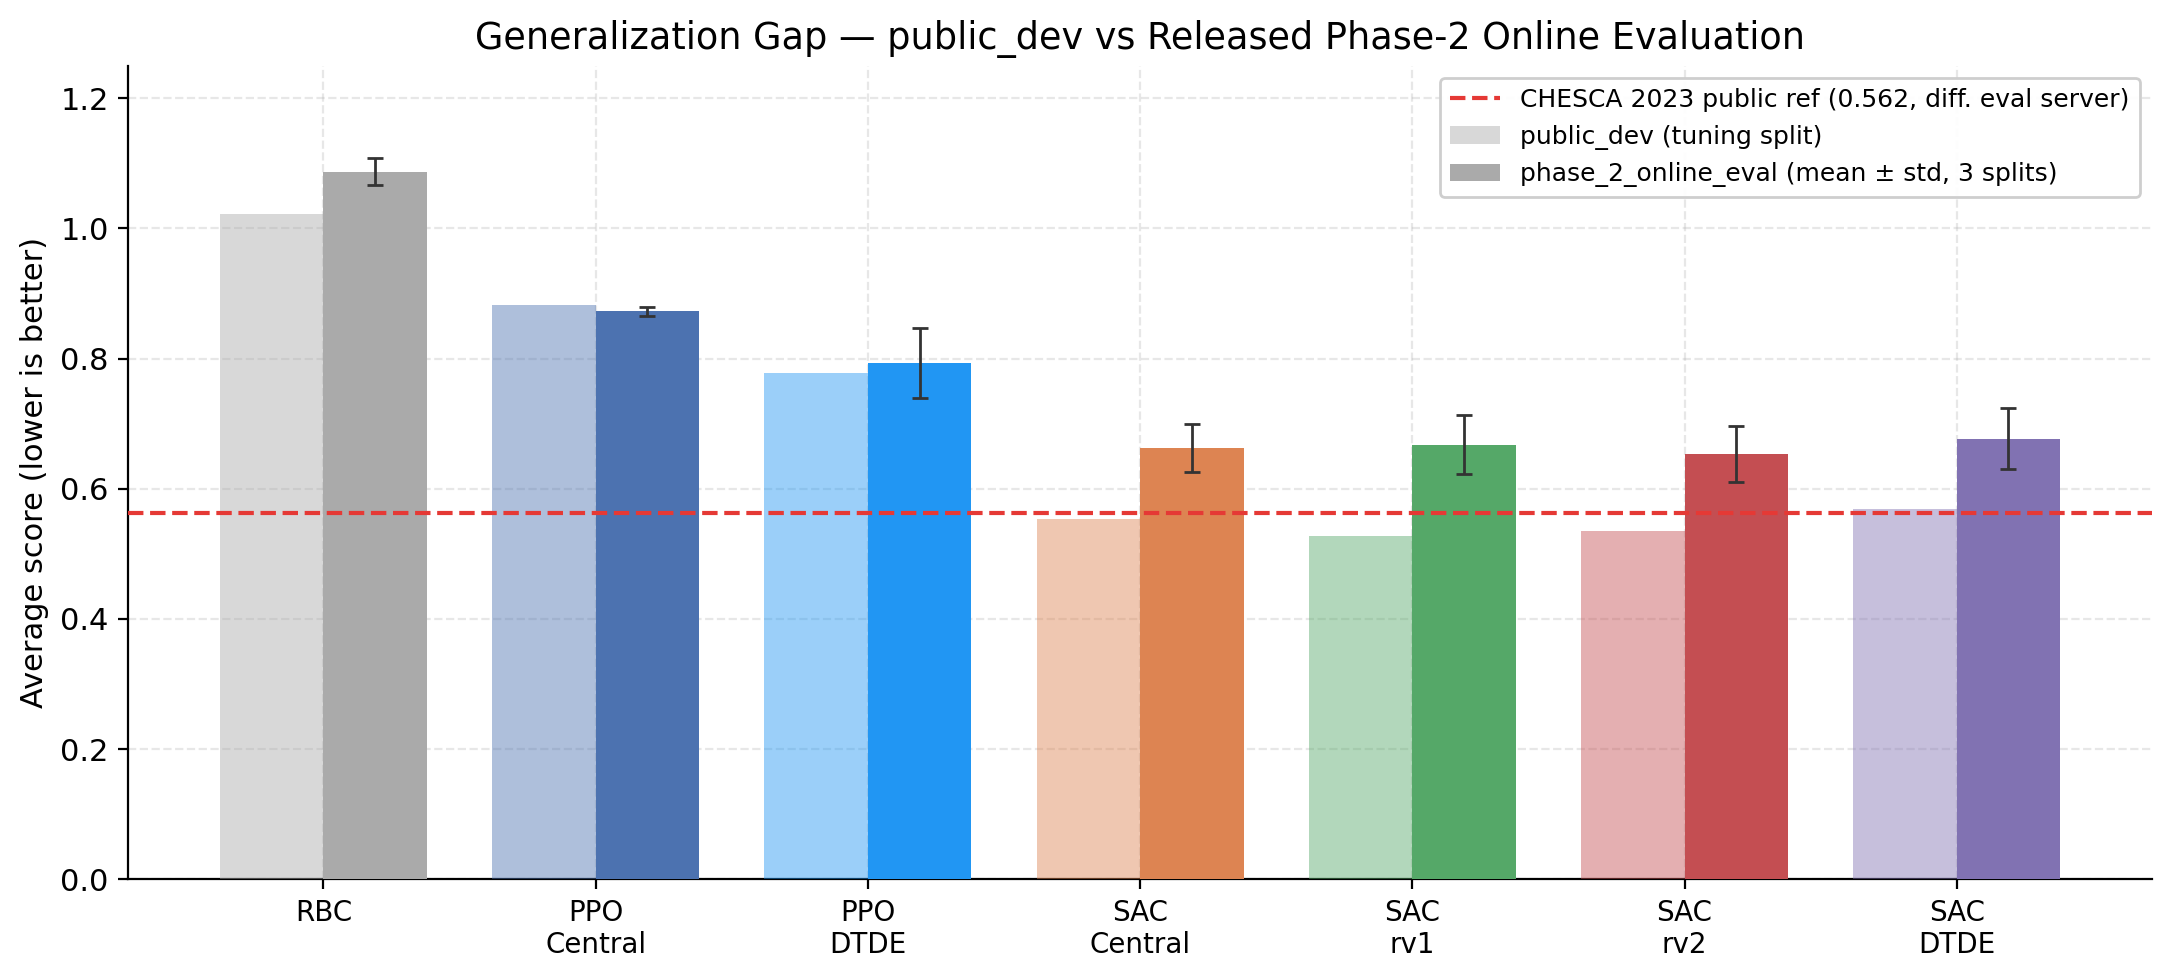
\includegraphics[width=\linewidth]{figures/generalization_gap.png}
    \caption{
        Generalization gap between the local \texttt{public\_dev} tuning split and the released \texttt{phase\_2\_online\_eval} mean for each method. SAC variants show modest, consistent degradation from local to held out; PPO shared-DTDE shows higher variance, confirming that SAC's stronger local policies also generalize more stably across weather and demand conditions. Smaller gaps indicate better cross split generalization.
    }
    \label{fig:gen_gap}
\end{figure}

\paragraph{KPI breakdown.} Figure~\ref{fig:kpi} disaggregates the local composite score into its constituent KPIs. The dominant improvement comes from thermal discomfort, which carries weight 0.30 in the scoring formula. The best SAC variants reduce the discomfort proportion from 0.944 (RBC) to below 0.020. This single term explains why all RL policies beat RBC substantially even when their cost and carbon reductions differ. Carbon emissions and electricity cost both fall by roughly 55\%. The main remaining weakness is thermal resilience (\texttt{one\_minus\_thermal\_resilience}). SAC centralized \texttt{reward\_v1} improves this term relative to RBC (0.290 vs.\ 0.454), but it remains a visible contributor. Optimization based methods such as CHESCA and MPC have a structural advantage here because they can plan over storage and resilience constraints with an explicit horizon rather than learning tradeoffs only from sampled trajectories.

\begin{figure}[h]
    \centering
    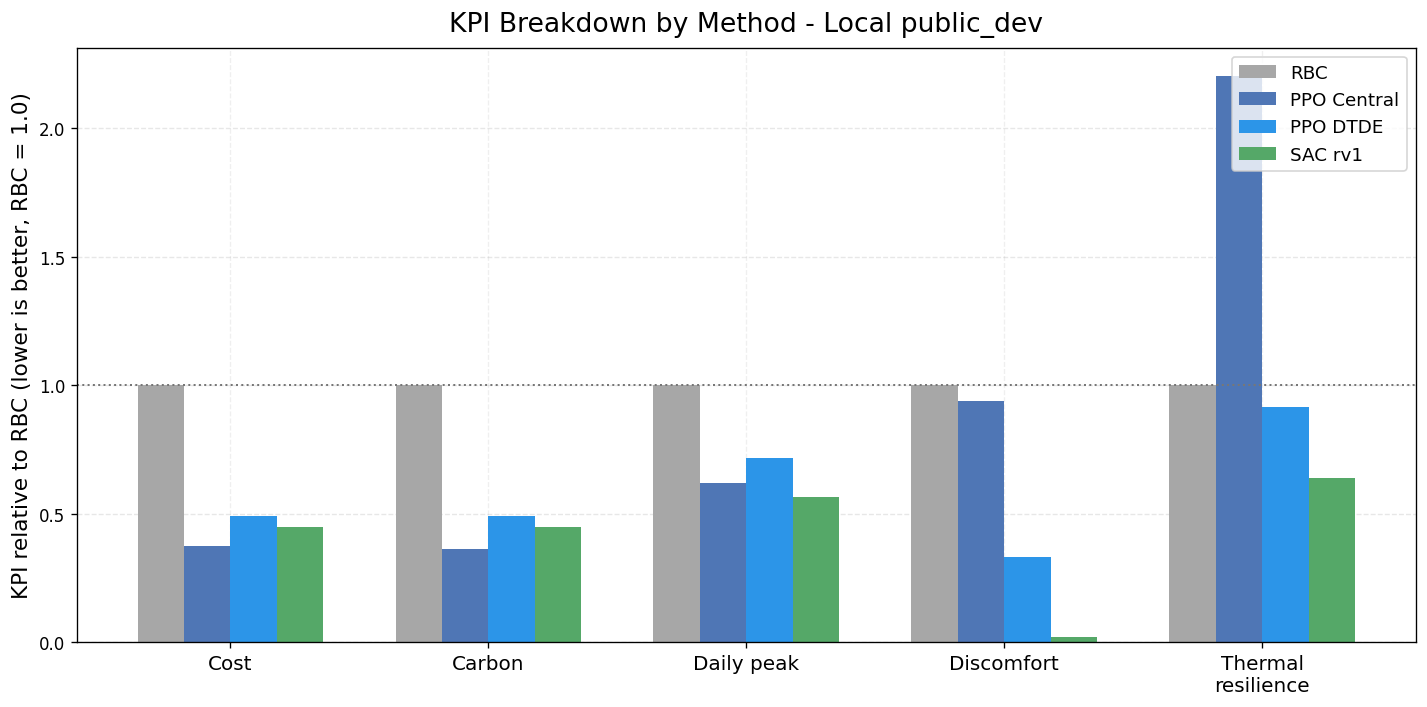
\includegraphics[width=\linewidth]{figures/kpi_breakdown.png}
    \caption{
        KPI-level breakdown for all methods on the local \texttt{public\_dev} split (lower is better). Thermal discomfort (rightmost bar) is the single largest source of improvement for all RL methods over RBC---the 0.30 weight on this term dominates the composite score and explains why even weaker RL variants substantially beat the heuristic baseline.
    }
    \label{fig:kpi}
\end{figure}

\paragraph{Reward design ablation.} Among centralized SAC variants, the baseline reward (\texttt{rv0}) is weakest locally at 0.554. \texttt{reward\_v1}, which mirrors the official 8 term weighting, achieves the best local mean at 0.527. \texttt{reward\_v2} is slightly worse locally (0.536) but leads on phase 2 (0.653 vs.\ 0.668 for \texttt{rv1}), supporting the hypothesis that smoothness penalties reduce local overfitting. The full KPI breakdown is in Table~\ref{tab:sac_ablation} in the Appendix. The most notable pattern is that the baseline reward produces the best thermal resilience (0.166 vs.\ 0.290--0.338), possibly because explicit KPI weighting redirects battery capacity away from resilience improving behavior.

\paragraph{PPO training dynamics.} Figure~\ref{fig:ppo_curve} shows shared-DTDE PPO learning curves for the learning rate sweep. Training is noisy but plateaus after roughly 1.5M steps; both learning rates converge to similar final levels (best seed mean, 0.783 vs.\ 0.796 for $10^{-4}$ and $3\times10^{-4}$ respectively). The seed variance ($\pm 0.037$) is large relative to the PPO--SAC performance gap ($\sim$0.25), so single seed PPO results would be easy to over interpret. Closing the gap to SAC would likely require changes to the observation model or credit assignment rather than a narrower learning rate sweep.

\begin{figure}[h]
    \centering
    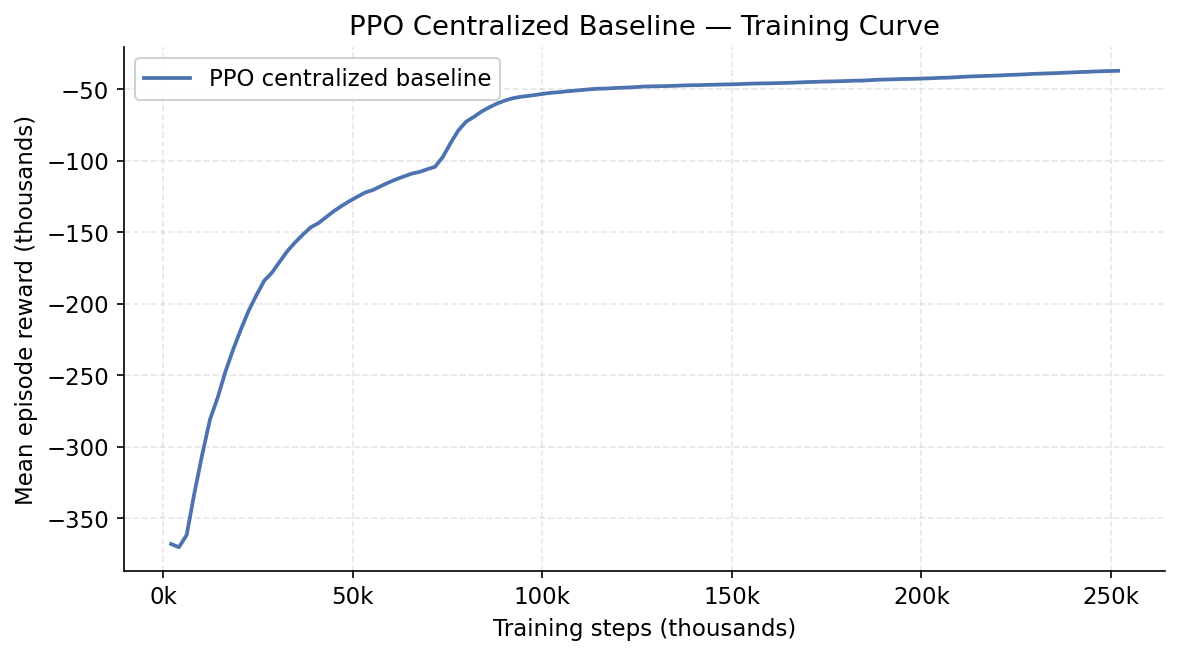
\includegraphics[width=0.75\linewidth]{figures/ppo_training_curve.png}
    \caption{
        PPO shared-DTDE training curves for both learning rates ($10^{-4}$ and $3\times10^{-4}$) across 10 seeds. Shaded bands are $\pm 1$ standard deviation. Training plateaus near 1.5M environment steps and seed variance is large relative to the PPO--SAC gap, motivating multiseed reporting over single run results.
    }
    \label{fig:ppo_curve}
\end{figure}

\section{Discussion and Limitations}\label{sec:discussion}

The results above establish that architectural portability is the binding constraint for real deployment, SAC substantially outperforms PPO in this continuous control setting, and RL baselines can close much of the gap to RBC through careful reward design and evaluation discipline, but remain below published optimization based winners. We discuss these limitations in more detail below.

\paragraph{Architectural portability is the primary design axis.} The cleanest finding is architectural rather than algorithmic. If deployment may involve a different number of buildings than training, a centralized policy is incompatible by construction, while a shared-DTDE policy transfers without any network changes. On 3 building splits, centralized SAC slightly outperforms shared-DTDE SAC; the cost of decentralization is a small local score penalty (~4 points absolute). Phase 3 reverses the ordering entirely. Shared-DTDE is the only topology that can produce a score at all (0.774 for SAC-DTDE vs.\ N/A for SAC centralized). Because real neighborhoods vary in size and a deployed system may be extended over time, practical RL controllers for building energy management should account for this portability constraint at design time rather than treating it as an afterthought.

\paragraph{SAC substantially outperforms PPO for this domain.} Across topologies and splits, SAC variants score roughly 15--25 percentage points below PPO variants. The most likely explanation is sample efficiency. SAC reuses historical transitions through off policy replay, and entropy regularization reduces sensitivity to reward scaling. PPO is simpler to implement. It avoids replay buffers and target networks, but that simplicity does not translate to better performance in continuous battery control where replay is directly beneficial.

\paragraph{Reward design matters within SAC.} The gap between the SAC baseline and \texttt{reward\_v1} (0.554 vs.\ 0.527 locally) shows that training on the official scoring objective outperforms training on a proxy. The smoothness penalties in \texttt{reward\_v2} trade a small local regression for better phase 2 generalization. Large SoC swings and repeated sign flips become costly even if they improve a short local trajectory, and this behavioral regularization transfers better when weather and demand traces change. For deployment on new buildings, \texttt{reward\_v2} is therefore the more robust choice. An important practical implication is that the reward design decision is inseparable from the evaluation protocol. If we had only measured performance on the local \texttt{public\_dev} split, we would have selected \texttt{rv1} as the best reward and missed the fact that \texttt{rv2} generalizes better. This underscores the value of held out evaluation even for design choices that appear secondary to algorithm selection.

\paragraph{Comparison to optimization based methods.} CHESCA achieved 0.562 on the official 2023 public leaderboard \citep{pinto2024citylearn}, below our best held out SAC result of 0.653 on the released phase 2 splits. This is benchmark context, not a head to head comparison. Our phase 2 results use the subsequently released evaluation datasets, not the original competition server, so a direct numerical comparison is not valid. Substantively, CHESCA and the HKUST solution \citep{zheng2025optimizing} use hierarchy to separate building level and community level objectives, giving them a natural way to reserve storage for future events and enforce resilience constraints. Our shared-DTDE policies gain portability by treating buildings as independent instances, but they give up the community level optimization layer. A natural next step is a hybrid controller that uses a learned per building policy for fast local proposals and an MPC or optimization layer to enforce aggregate grid and resilience constraints. Combining the portability of shared-DTDE with the explicit planning structure of the top leaderboard entries.

\paragraph{Limitations.}
\begin{itemize}
    \item Single tuning split. All reward variants and hyperparameters were selected on the local \texttt{public\_dev} split. A stronger protocol would reserve a separate validation split to reduce the risk of overfitting design choices to one dataset.
    \item Compute constraints. SAC shared-DTDE was run with only 3 seeds (pilot), and the reward variant ablation was not conducted for PPO due to GPU budget limits. The PPO sweep covered 10 seeds but only two learning rates; wider sweeps might yield better configurations.
    \item Centralized policies not portable. The centralized SAC variants, which achieve the best local scores, cannot be evaluated on phase 3 (6 building) splits. Generalization claims for centralized SAC are necessarily limited to same topology held out sets.
    \item No forecast model. We use only the short horizon forecasts provided by the environment. A learned demand prediction module could improve policy quality and is a common component of strong model predictive baselines.
    \item CHESCA comparison is indirect. The 0.562 CHESCA reference is from the competition paper \citep{pinto2024citylearn} and was scored on a hidden split via an evaluation server that is no longer publicly accessible, making a direct numerical comparison impossible.
\end{itemize}

{\footnotesize
% \paragraph{Acknowledgements.} We thank XXX.

\bibliographystyle{apalike}
\bibliography{references}
}

\section*{Appendix}

\paragraph{Per-split generalization table.}

Table~\ref{tab:cross_split} reports the per split composite scores used in Figure~\ref{fig:per_split}. Entries marked ``---'' indicate that a method cannot execute on that split (centralized policies on phase 3) or that results were not collected.

\begin{table}[h]
\centering
\small
\begin{tabular}{lccccccc}
\toprule
\textbf{Method} & \textbf{public\_dev} & \textbf{p2\_e1} & \textbf{p2\_e2} & \textbf{p2\_e3} & \textbf{p3\_1} & \textbf{p3\_2} & \textbf{p3\_3} \\
\midrule
RBC                & 1.023 & 1.109 & 1.085 & 1.068 & 1.117 & 1.124 & 1.100 \\
PPO Central        & 0.883 & 0.881 & 0.868 & 0.870 & --- & --- & --- \\
PPO DTDE           & 0.777 & 0.829 & 0.813 & 0.738 & 0.846 & 0.844 & 0.840 \\
SAC Central        & 0.554 & 0.684 & 0.687 & 0.615 & --- & --- & --- \\
SAC \texttt{rv1}   & 0.527 & 0.707 & 0.686 & 0.611 & --- & --- & --- \\
SAC \texttt{rv2}   & 0.536 & 0.691 & 0.670 & 0.597 & --- & --- & --- \\
SAC DTDE           & 0.569 & 0.715 & 0.700 & 0.615 & 0.786 & 0.762 & 0.775 \\
\midrule
CHESCA (ref.)      & --- & 0.562 & --- & --- & --- & --- & --- \\
\bottomrule
\end{tabular}
\caption{Per-split composite scores ($\downarrow$ better). Phase-2 columns (p2\_e1--p2\_e3) are the released online-evaluation splits; phase-3 columns (p3\_1--p3\_3) are the 6-building held-out splits. CHESCA is the 2023 competition winner reference from \citet{pinto2024citylearn}, evaluated on the original competition server (different split; shown for context only).}
\label{tab:cross_split}
\end{table}

\paragraph{SAC reward-variant ablation detail.}

Table~\ref{tab:sac_ablation} extends the local SAC comparison with KPI-level columns. All SAC variants reduce thermal discomfort from the RBC level of 0.944 to near zero ($\leq 0.020$), consistent with the 0.30 weight on this term. The SAC baseline achieves a similar reduction despite not explicitly weighting discomfort, suggesting that the net-consumption proxy also indirectly rewards occupant comfort. Differences across variants are most visible in thermal resilience (0.166 vs.\ 0.290--0.338), where the baseline reward outperforms the shaped variants.

\begin{table}[h]
\centering
\small
\begin{tabular}{lccccc}
\toprule
\textbf{Variant} & \textbf{Score} & \textbf{Cost} & \textbf{Carbon} & \textbf{Discomfort} & \textbf{1$-$Resilience} \\
\midrule
SAC baseline (\texttt{rv0}) & 0.554 & 0.888 & 0.904 & 0.012 & 0.166 \\
SAC \texttt{rv1}            & 0.527 & 0.823 & 0.848 & 0.019 & 0.290 \\
SAC \texttt{rv2}            & 0.536 & 0.811 & 0.836 & 0.020 & 0.310 \\
SAC shared-DTDE \texttt{rv2} & 0.569 & 0.809 & 0.829 & 0.023 & 0.338 \\
\midrule
Local RBC                   & 1.023 & 1.839 & 1.890 & 0.944 & 0.454 \\
\bottomrule
\end{tabular}
\caption{SAC reward-variant ablation on local \texttt{public\_dev}. KPI columns are seed-averaged means (lower is better). ``Cost'' and ``Carbon'' are normalized district totals; ``Discomfort'' is the proportion of occupant-hours with comfort violations; ``1$-$Resilience'' is the proportion of hours without full thermal resilience.}
\label{tab:sac_ablation}
\end{table}

\end{document}
